\section{Evaluation}
\label{sec:eval}

We evaluate RCuckoo by directly comparing its performance in terms of
throughput and latency against representative state-of-the-art
disaggregated key/value stores.  When accessing sufficiently large values, all
systems can max-out our testbed's 100-Gbps
link rate, so we focus on workloads with small key/value pairs that
remove the bandwidth limitation, exposing the (in)efficiency of each
system's management and synchronization techniques.

When values are stored inline, RCuckoo outperforms existing systems while delivering competitive
insert latencies.  Using fault injection, we show that our distributed approach to client failure
detection and recovery enables RCuckoo to sustain high throughput even though 100s of clients are
failing per second.  Finally, we justify our design decisions through a series of micro-benchmarks.
Specifically, we quantify the benefit RCuckoo extracts from its locality enhancement
%% %and speculative search strategy %
before measuring the impact of
%conduct sensitivity analysis of our choice of locality parameter, covering read threshold, and
index-table entry size.

\section{Implementation}

Our implementation of RCukcoo consists of a of 8.7k C++
implementation and a 12k line Python implementation which
simulates RDMA. Both implementations will be made available
on Github.  All results reported in Section~\ref{sec:eval}
are from the C++ implementation. At the time of writing only
the python implementation includes support for delete
operations, and extent entries. As such all C++ results are
for inserts, reads, updates and inlined table operations.
RCuckoo is designed for ConnectX-5 NICs. It uses OFED-4.9
which supports experimental verbs for atomic masked CAS and
device mapped memory. 


\begin{figure*}[ht]
  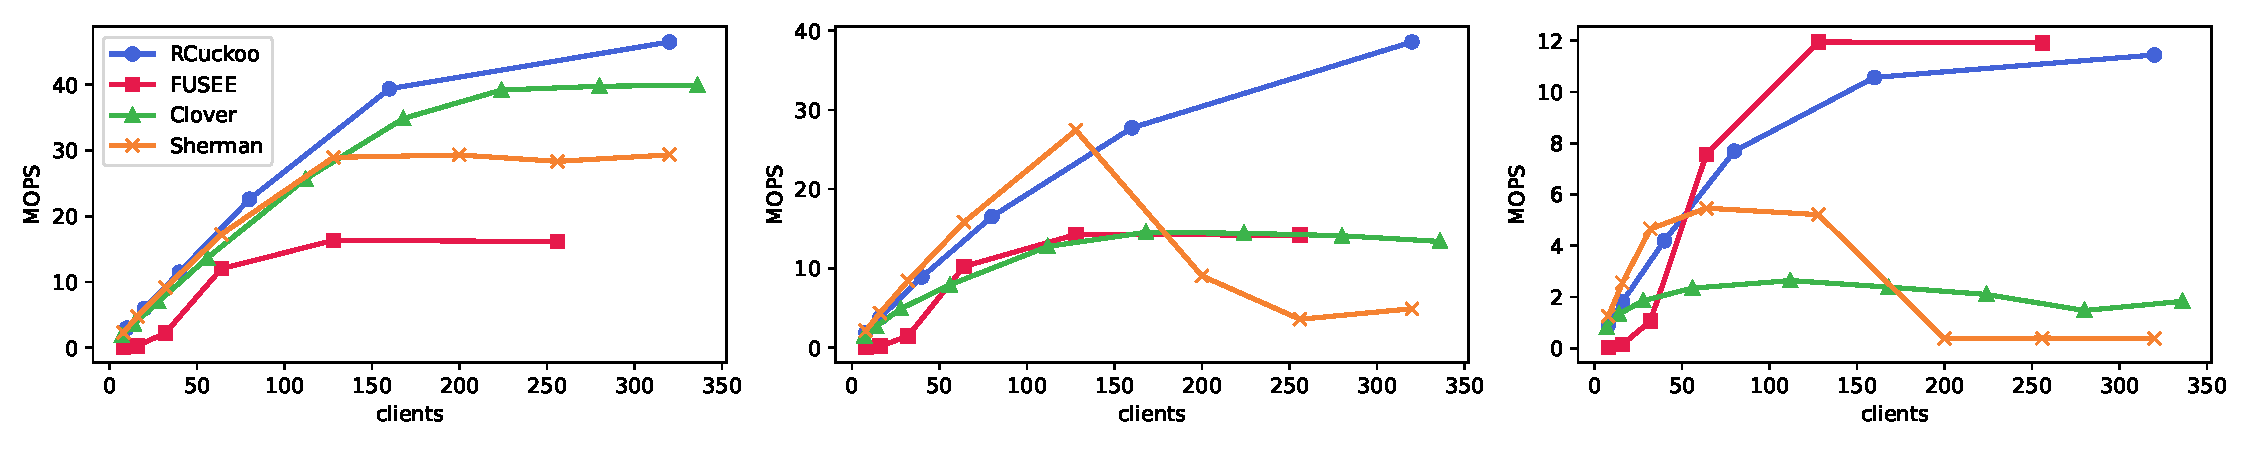
\includegraphics[width=0.99\linewidth]{fig/hero_ycsb_throughput.pdf}
  \vskip -1em
\caption{Throughput as a function of the number of clients for three different workloads (Zipf $\theta$=0.99): \textbf{(a)} Read only (YCSB-C), \textbf{(b)} YCSB-B 95\% read, 5\% update and \textbf{(c)}
    50\% read 50\% update (YCSB-A).}
\label{fig:ycsb_throughput}
\vskip -1em
 \end{figure*}


\subsection{Testbed}

We conduct our evaluation on an 9-node cluster of dual-socket Intel
machines. Each CPU is an Intel Xeon E5-2650 clocked at
2.20~GHz. Each machine has 256~GB of RAM with 128~GB per NUMA
node. All machines have a single dual-port ConnectX-5 attached to a
100-Gbps Mellanox Onyx switch. In our RCuckoo experiments we use one
sever as the memory server and the rest a client machines
spreading threads evenly across machines.

%\subsection{Comparison systems}

We compare RCuckoo against three recent RDMA key/value stores with
different designs, FUSEE~\cite{fusee}, Clover~\cite{clover}, and
Sherman~\cite{sherman}.  While none have the exact same assumptions or
feature set as RCuckoo, each represents an apt comparison point for
different aspects.  To avoid biasing our evaluation, we consider the same
workloads (YCSB) as the authors of the previous systems.
%
%We directly compare RCuckoo against three disaggregated
%key-value stores  Each system has distinct design
%tradeoffs. 
%%
%%
%%

\textbf{FUSEE} is a fully disaggregated key/value store that
represents the closest available comparison point to RCuckoo.  While
both employ only 1-sided RDMA operations, FUSEE eschews locking in
favor of optimistic insertions.  FUSEE clients use CAS operations
to manage fixed, 64-bit index table entries that contain pointers to
values stored in extents.  Due to its reliance on CAS operations, FUSEE is unable to support inlined storage of small
values like RCuckoo, forcing all reads to require two round trips.
%Fusee is the closest comparison we have to illustrate
%the tradeoffs between locks and optimistic concurrency.
%is a key-value store designed for full
%disaggregation~\cite{fusee}.  It is built on top of RACE~\cite{race}
Unlike RCuckoo, FUSEE is designed to support replication.  To remove the overhead of replication, 
%While RACE represents a more direct comparison to RCuckoo, no open
%source implementation of RACE is available.  Instead,
we deploy FUSEE with a single memory node.
%FUSEE/RACE hashing uses fixed-sized 64-bit index entries
%to in order to employ RDMA compare-and-swap operations for updates. As
%such, RACE-based systems cannot store key-value pairs in the index
%table itself and require a second round trip even for reads of small values.
%on reads to recover
%extent entries which contain full key value pairs.

\textbf{Clover} is only partially disaggregated---it requires a
metadata server to manage its index structure---but can deliver higher
read performance than FUSEE on read-only workloads.  Clover is
designed to leverage remote persistent memory and implements both
reads and updates using one-sided RDMA operations.  Moreover, unlike
FUSEE---and similar to RCuckoo---Clover reads are self verifying.
%Clover uses index caching to optimize reads.  When re-reading key-value
%entries clover can as it directly
%reads the entry without negotiating with the index.
In contrast to prior comparisons~\cite{fusee} that force
clients to consult the metadata server on each read, we allow Clover
to take advantage of its client caching to achieve maximum performance
on read-heavy workloads.

%% Clover is a partially disaggregated system which uses
%% two-sided RDMA operations to modify the index and one-sided
%% operations for updates, deletes, and reads.

%% Sherman a disaggregated B-Tree and the only system at the
%% time of writing which uses locks and not optimistic
%% concurrency to guard its index. Our performance comparison
%% with Sherman is not apples to apples. Sherman maintains
%% ordered key-value pairs for range queries and thus has
%% higher overheads on updates than the other systems.

\textbf{Sherman} is the highest-throughput distributed key/value
storage system of which we are aware that employs locks.  Sherman
maintains a B-tree that spans multiple servers and supports range
queries, a feature none of the other systems---RCuckoo
included---provide.
%is a B-tree designed for remote memory~\cite{sherman}.
%and high write
%throughput.
%Unlike Clover and FUSEE which employ optimistic consistency control,
%Sherman uses locks to guard updates similar to RCuckoo.
On the other
hand, Sherman clusters are not fully disaggregated: each node in a
cluster is a peer with many CPU cores and a single memory core
that is responsible for servicing allocation RPC calls from clients.
%Unlike the other systems
%Sherman is cluster based, and does not support a having
%isolated memory machines.
%All machines are equal nodes in a
%cluster and run both a memory controller and client threads.
As such, Sherman does not encounter the same bandwidth bottlenecks as
the other systems because requests are partitioned across
%all machines in the cluster.
machines.
%However, it assumes that collocated clients can resolve lock
%contention locally and clients collocated with their segment
%of the B-Tree can perform local operations. These
%assumptions enable Sherman to have high performance under
%contention even though it uses locks and manages a more
%complex data structure than the unordered key-value stores.
%While Sherman does not meet the fully disaggregated model it
%does provide a good comparison for RCuckoo as it is the only
%other system to use locks in remote memory.


% \subsubsection{Clover}
% \todo{insert a short clover description}

\begin{figure*}[ht]
    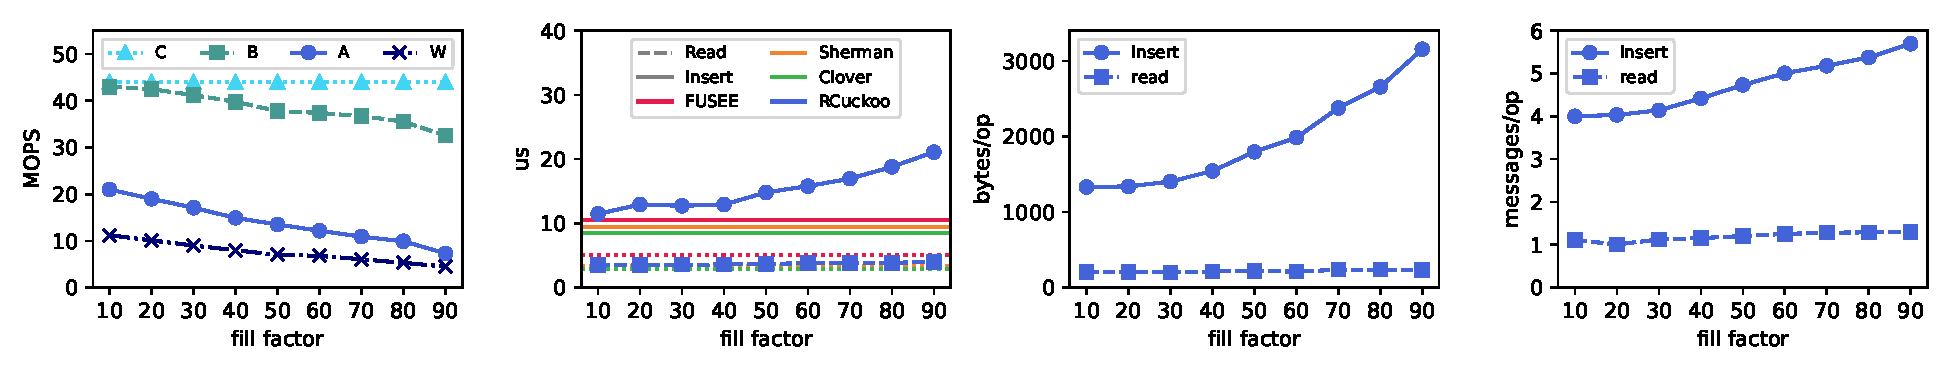
\includegraphics[width=0.99\linewidth]{fig/hero_ycsb_fill.pdf}
\vskip -1em
    \caption{Insert performance as a
    function of fill factor. \textbf{(a)} Throughput for four different insert workloads, \textbf{(b)}
    median operation latency, \textbf{(c)} mean operation size, and \textbf{(d)}
    mean per-operation RDMA message count under workload A.}
\vskip -1em
    \label{fig:ycsb_fill}
\end{figure*}

% \begin{figure}[ht]
%     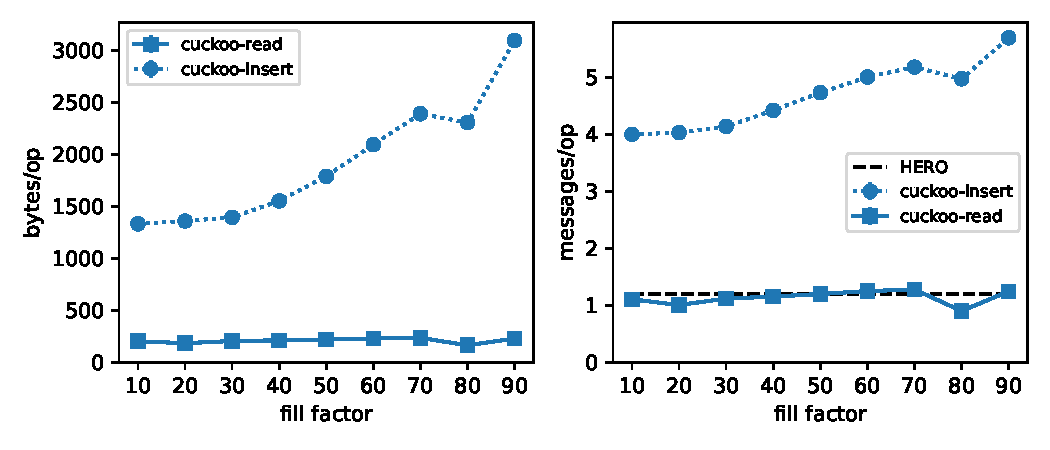
\includegraphics[width=0.99\linewidth]{fig/hero_ycsb_fill_ops_bw.pdf}
%     \caption{YCSB-A workload messages and bandwidth per operation as a function of fill factor}
%     \label{fig:ycsb_fill_ops_bw}
% \end{figure}



\subsection{Performance}

We start by considering throughput and latency on the classical YCSB
workloads which employ varying mixes of read and update operations
before turning to the more complex insert operation.  RCuckoo delivers
the highest performance on reads and updates across all settings,
while insert performance varies as a function of table fill factor.
Even in the worst case, however, RCuckoo limits I/O amplification to
around 2$\times$.
\todo{What is the row/read size?  How close are we
  to line rate?}

\textbf{Throughput.} Figure~\ref{fig:ycsb_throughput} shows YCSB
throughput for RCuckoo, FUSEE, Clover, and Sherman on three different
YCSB workloads. For each system, we allocate a 100-M-entry table and
pre-populate it with 90~M entries that each consist of a 32-bit key
and 32-bit value (we consider larger sizes in Section~\ref{ss:mb}).
We plot the aggregate throughput of a variable number of clients
concurrently accessing entries according to a Zipf(0.99) distribution.

In a read-only (YCSB-C) workload, FUSEE suffers from its extent-based
value storage.  RCuckoo, Clover, and Sherman perform similarly at
low-to-moderate levels of concurrency, but they separate at scale.
Sherman's read algorithm is more complex than RCuckoo's leading to
lower top-end performance.  Clover's client-side caching shines under
this skewed workload, where almost all reads hit in a client's index
cache, requiring only a single read for the value; its performance
degrades under a more uniform workload (not shown).  RCuckoo, on the
other hand, reads inlined values in a single round trip
regardless of the distribution, leading to the highest performance.


Increased update rate slows all systems.  Even with only 5\% updates (YCSB-B), the picture changes
dramatically.  Sherman performs well at low levels of concurrency due to its
single-round-trip reads, but hits a severe bottleneck due to lock contention on the skewed access
pattern.  (Sherman improves---but does not surpass RCuckoo---for uniform workloads,
not shown, where lock contention is less of an issue.) Caching is less effective with updates,
bringing Clover's throughput in line with FUSEE.
%performs similarly to FUSEE on YCSB-B; we suspect that with tuning Clover's read-only performance
%could be brought to par with RCuckoo.  , and is the most competitive with RCuckoo in read-only
%scenario.  When it is able to leverage its client index cache,

On the 50/50-mixed YCSB-A workload RCuckoo and FUSEE perform
similarly, although we are unable to scale FUSEE past 250 clients in
our testbed while RCuckoo continues to scale.
%begins to surpass FUSEE after about 125 clients.  FUSEE's maximum performance is gated by its requirement for an additional round trip per operation (to
%retrieve the extent).
Sherman begins to suffer from lock contention even earlier, topping
out around 5 MOPS before collapsing.  (Absolute performance improves as Zipf skew decreases---not shown---but the
trend remains.)
Clover performs worst under
write-heavy workloads due to its inability to effectively leverage
caching with a constantly changing index structure.

%On read-mostly (YCSB-B) and read-only (YCSB-C) workloads RCuckoo
%pulls ahead.
%, extracts even further benefit from its ability to complete
%reads in a single round trip by collapsing most reads into a single
%RDMA request (Section~\ref{sec:read_threshold}).
%  While lock contention is not an issue in the read-only YCSB-C,



\begin{figure*}[t]
    \centering
    % \begin{subfigure}{0.24\linewidth} % original width for 4 figures
    % \newcommand{\subfigwidth}{0.24\linewidth}
    \newcommand{\subfigwidth}{0.24\linewidth}
    \begin{subfigure}{\subfigwidth}
      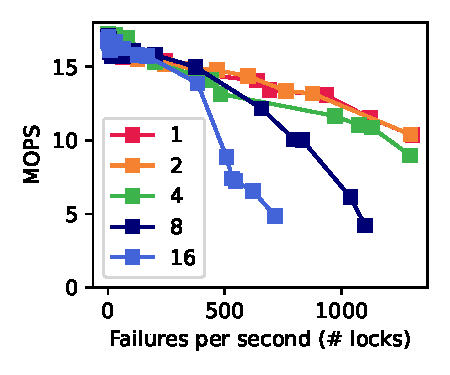
\includegraphics[width=0.99\linewidth]{fig/fault-rate.pdf}
          \end{subfigure}
    \begin{subfigure}{\subfigwidth}
        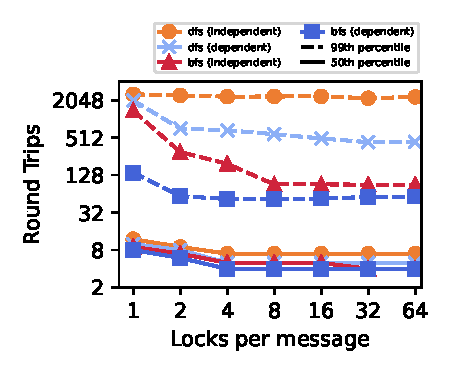
\includegraphics[width=0.99\linewidth]{fig/search_dependence.pdf}
        % \label{fig:hash_fill}
        % \caption{}
    \end{subfigure}
    % \begin{subfigure}{\subfigwidth}
    %     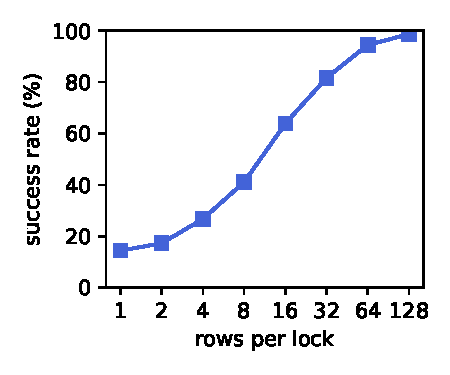
\includegraphics[width=0.99\linewidth]{fig/search_success_lock_size.pdf}
    % \end{subfigure}
    %\begin{figure}[ht]
    \begin{subfigure}{\subfigwidth}
      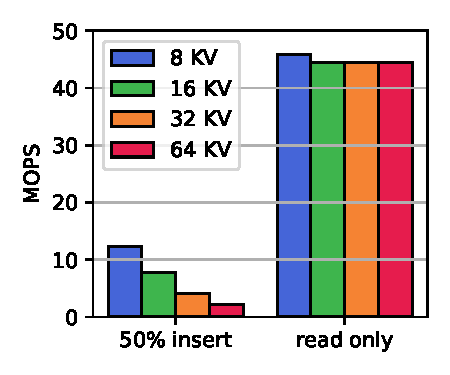
\includegraphics[width=0.99\linewidth]{fig/entry_size.pdf}
          \end{subfigure}
    \begin{subfigure}{\subfigwidth}
      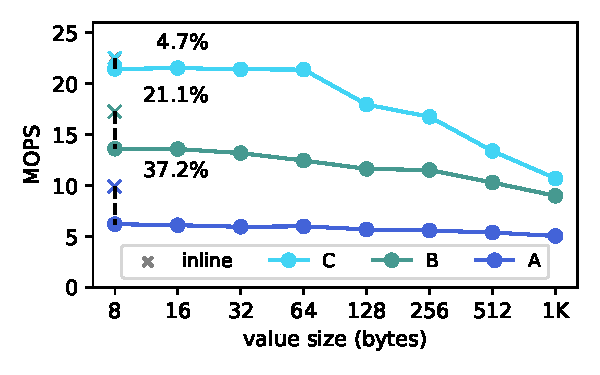
\includegraphics[width=0.99\linewidth]{fig/extent.pdf}
          \end{subfigure}
\vskip -1em
    \caption{RCuckoo microbenchmarks:
      \textbf{(a)} YCSB-A throughput vs. client failure rate,
          \textbf{(b)} round trip times required to acquire locks on insert,
%    \textbf{(c)} insert second-search success rate as a function of lock granularity, and
    \textbf{(c)} throughput vs. key/value-entry size for 50\% insert 50\% read,  and YCSB-C (read-only) workloads, and
    \textbf{(d)} extent performance for value sizes up to 1~KB. Dashed line marks the inline performance on 16 Byte entries. Overheads marked in black.
    }
    % \label{fig:microbenchmarks}
             \label{fig:microbenchmarks}
\vskip -1em
\end{figure*}

\textbf{Insert performance}

Despite its complexity, RCuckoo's insert operation remains highly performant.  To evaluate insert
performance we run workloads with a mix of reads and inserts.  Figure~\ref{fig:ycsb_fill} considers
RCuckoo's performance on workloads that exclusively use inserts (rather than updates); as with YCSB
nomenclature A is 50\% insert and 50\% read; W is insert only. Inserts become more expensive as the
table fills, so we pre-populate the table with a varying number of entries and report insert
performance as a function of the table's initial fill factor.
%%
\todo{How long/how many inserts are
performed?}

As a baseline we collect the read and insert latencies for all systems under light load
(Figure~\ref{fig:ycsb_fill}(a)). Read latency is nearly identical for all systems save FUSEE as it
makes a read to both the index and extent. Insert times vary: Clover and Sherman use two-sided RDMA
operations for insert and both need to perform allocations and set up metadata for the requesting
client.  FUSEE is slightly slower, roughly the same as RCuckoo's best case.  As the table fills,
however, cuckoo paths grow in length causing RCuckoo insert operations to require additional round
trips to find valid cuckoo paths.  At maximum fill, insert operations take roughly twice as long as
in an empty table. 

Figure~\ref{fig:ycsb_fill}(b) shows impact of table fill on insert throughput (320 clients). As the
index table fills, cuckoo paths become longer leading to increased contention and additional
bandwidth consumption from larger covering reads. In each case (except read-only C) RCuckoo's
performance declines with fill factor. In the insert-only W case RCuckoo's performance drops from a
high of 11.5 MOPS in a nearly empty table to 4.5 MOPS at a 90\% fill factor.  As a point of
comparison, FUSEE's maximum insert-only performance is 9.1 MOPS on our testbed, although it is
independent of fill factor.  While FUSEE out-performs RCuckoo at high fill factors, we observe that
insert-only workloads are rare in practice~\cite{facebook-memcached}.
%%
Figures~\ref{fig:ycsb_fill}(c) and (d) show the impact of fill factor on the bandwidth cost of each
operation and the number of RDMA messages they require to complete.

% \begin{figure}[t]
%     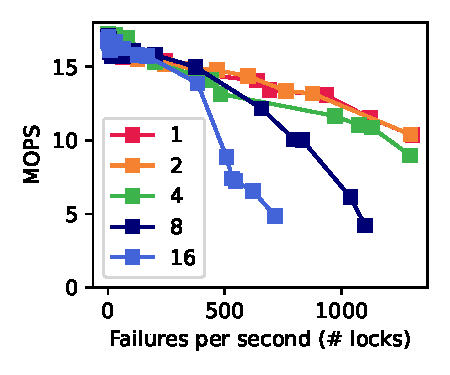
\includegraphics[width=0.99\linewidth]{fig/fault-rate.pdf}
%     \caption{YCSB-A throughput vs. client failure rate.}
%     \label{fig:failure_throughput}
%     \vskip -1em
% \end{figure}

\subsection{Fault tolerance}


RCuckoo runs at nearly full throughput during realistic
failure scenarios and remains functional in the face of
hundreds of failures per second.
%When a client fails while
%holding a lock the lock is stranded and requests for that
%lock will block until after a client times out and reclaims
%the lock.
%%
We emulate client failures by
performing a partial insert operation that randomly truncates the
batch of RDMA operations including lock releases, leaving the table
%. The table
%entries are left
in one of the  states listed in
Section~\ref{sec:table-repair}.
%and locks are left set.
Figure~\ref{fig:microbenchmarks}(a) shows that
%illustrates RCuckoo's
%ability to operate at high throughput in the face of
%failures.
%Lock granularity increases the probability that
%multiple clients will block on the same failed lock. Larger
throughput remains high until about 500 client failures per second, at
which point lock granularity begins to play a significant role;
finer-grained locks are easier to recover leading to less throughput
degradation.
%locks have little difference when failures are semi-frequent
%and have a larger impact as hundred of failures occur per
%second.  The performance impact of a few number of failures
%per second is low which is ideal considering that failures
%in RDMA clusters are relatively rare.
As a point of reference, we observe that RDMA itself struggles to handle churn of this magnitude:
%RCuckoo can still operate despite
%thousands of failures per second while
a server can only
establish approximately 1.4~K RDMA connections per second~\cite{xrdma}.
%using state of the art techniques~\cite{xrdma}.

\subsection{Microbenchmarks}
\label{ss:mb}

Having established RCuckoo's superiority over prior systems and
demonstrated its robustness to client failure, we now evaluate the
impact of particular design choices.





% \begin{figure}[t]
%     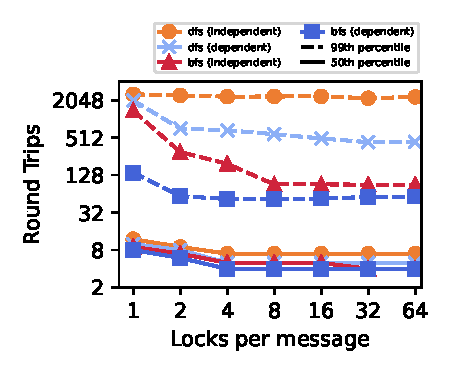
\includegraphics[width=0.99\linewidth]{fig/search_dependence.pdf}
%     \caption{Round trips per insert operation with independent
%     and dependent hashing.  (Note log-scale axes.)}
%     \label{fig:search_dependence}
% \end{figure}
%Hash dependence and search function choice have the highest
%impact on RCuckoo's performance. Dependent hashing reduces
%the probability locks are scattered throughout the table
%which enables RCuckoo to combine lock requests into a few
%masked CAS messages. Simultaneously search function choice
%dramatically affects the length of cuckoo paths.

\textbf{Locality enhancement.}
Figure~\ref{fig:microbenchmarks}(b) illustrates the dramatic benefit
RCuckoo extracts from its dependent hashing combined with a BFS
cuckoo-path search strategy.  To focus on longer cuckoo paths, we
pre-populate a 100-M entry table to 85\% and then report both the median
and 99th percentile round trips per insert 
key/value pairs until the table is 95\% full as a function of lock
granularity.  While median performance is on the same order, the
99th-percentile insert takes an order of magnitude fewer round trips
with dependent hashing and BFS as opposed to independent hashing and
DFS as used in prior cuckoo hash
systems~\cite{cuckoo-improvements,pilaf,cuckoo}.  As before
(c.f. Figure~\ref{fig:cuckoo-problems}), performance is similar with
four or more locks per message.

%% We vary the number of locks per message to demonstrate the
%% effect of path length and show why masked cas plays an
%% important role in RCuckoo's performance. We measured both
%% the median, and 99th percentile round trips per request on a
%% table with 100M entries. We fill the table to 85\% and then
%% executed insert operations to 95\%.

%% DFS with no hash dependence has extremely poor performance
%% at it's tail, taking over 2K round trips to complete. Both
%% at it's median and 99th percentile it sees only small
%% benefits from setting multiple locks per request as the
%% locks are scattered throughout the table. DFS with
%% dependence has far lower tail latency, and improves the
%% number of locks which can be acquired per message, however
%% it still constructs long rather than minimum length paths.
%% BFS with dependence provides the best performance and gains
%% the most from setting more locks per request. At 64 locks
%% per request it has 7.5x lower round trips at it's 99th
%% percentile and 4 rather than 5 round trips on average. We
%% found that A* search provided the same minimal path length
%% as DFS with slightly better locality. It's performance
%% against BFS was only superior at fill factors above 95\% and
%% lower elsewhere due to a higher runtime cost on short paths.



% Hash function locality hash a major impact in RCuckoo's
% performance.  Acquiring locks can only be done in a few
% round trips when the locks are clustered together tightly in
% the lock table.  Furthermore, the search function used to
% determine the cuckoo path has a large impact on the locality
% of the locks necessary to lock the path. We evaluate
% dependent hashing and independent hashing as well as random
% and a* search. We measure the number of round trips required
% for each control as a function of the number of locks which
% can be acquired per round trip.

% Figure~\ref{fig:search_dependence} shows the performance
% improvements gained by both locality hashing and A* search.
% In this experiment the table is filled from 0 to 90\% full
% with a YCSB-w workload. We measure the 99th percentile of
% round trips for these workloads. Random search with
% independent hashing leads to a large number of round trips
% as locks are scattered throughout the table. RDMA masked CAS
% operation do little here to reduce the round trips as they
% can rarely acquire more than one lock in a round trip. With
% dependent hashing and random search RDMA CAS operation are
% almost sufficient to reduce round trips, however the absolute
% number of locks required per insert is high which leads to
% greater contention. A* search with dependent hashing has
% cuckoo paths that are both short, and clustered together.



% \label{sec:search_success}
% \begin{figure}[t]
%     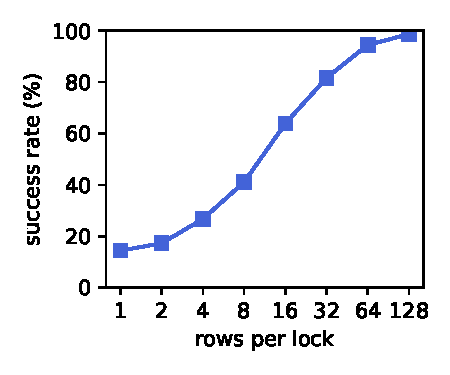
\includegraphics[width=0.99\linewidth]{fig/search_success_lock_size.pdf}
%     \caption{Failure rate of search algorithms vs. lock size under high contention}
%     \label{fig:search_success}
% \end{figure}

% \textbf{Secondary search.}
% We measure second search success rate as a function of lock granularity under high contention.  A
% table is filled up to 85\% and then 320 clients concurrently run an insert-only workload.  For this
% experiment only, we flush the client's cache before every insert, ensuring the initial speculative
% path will fail unless the entry does not require cuckooing (unlikely at this fill factor).
% Figure~\ref{fig:microbenchmarks}(c) plots the success rate of the second search as a function of
% lock granularity.  \todo{not sure how 99th percentile impacts things} Recall that if a second search
% fails, RCuckoo clients release their locks and retry the insert operation using the contents of
% their cache, so multiple speculative and secondary searches may be performed.  At one row per lock,
% secondary search has limited effectiveness (as the only alternative is to cuckoo a different set of
% entries among the same rows), leading to multiple retries (approaching 4 in the 99th percentile, not
% shown).  As locks cover additional rows, however, the second search becomes much more
% useful.
% At 64 rows per lock the second search succeeds 95\% of the time.


%% \subsubsection{Masked CAS}

%% Under contention masked CAS operations provide a significant
%% performance improvement. We measure it's benefit in terms of
%% throughput by comparing it with default CAS. In the
%% default case, when acquiring locks clients set the lock bits
%% for the locks they require and set all other bits in the CAS
%% to 0. If the CAS fails the current state of the lock table
%% over that range is returned as a result to the client and
%% the client tries to acquire their locks again using the
%% updated state of the lock table. Masked compare and swaps
%% are issued with the minimal mask required to set the locks.

%% Figure~\ref{fig:performance_breakdown} shows the improvement
%% gained by masked CAS. Default CAS operations perform better
%% with fewer rows per lock, as the probability of a lock being
%% set within the 64bit range is at its lowest. At higher rows
%% per lock CAS suffers from failed lock acquisitions from both
%% contested locks and due to a lack of synchronization. In
%% contrast masked CAS sees an improvement when two rows per
%% lock are used, as more second search attempts succeed, and
%% only suffers from direct lock contention as the rows per
%% lock increase.


% Figure~\ref{fig:performance_breakdown} plots the sensitivity of
% RCuckoo performance to various parameter settings.


\textbf{Entry/value sizes.} \label{sec:entry_size} 
%%
Inlined key/value entries enable single-round-trip
reads. However large entries increase bandwidth consumption for inserts.
% , so the larger the entries, the fewer values that require a second round trip.  
% However, for a
% fixed row size, larger entries imply fewer entries per row, increasing cuckoo path lengths (when
% measured in terms of rows).
%%
%, impacting insert performance.  % but larger values must be stored in extents.  % at the cost of
%inflating the bandwidth of % operations. We run a 50\% read 50\% insert and a read only % workload
%to illustrate the overhead of larger entries.
Figure~\ref{fig:microbenchmarks}(c) shows the effect of entry size on throughput under 50\% insert
and read-only (YCSB-C) workloads. Insert is a bandwidth-limited operation,
%quickly saturates the network bandwidth. At
%at 16-B entries link capacity restricts throughput to 8 MOPS. The performance of
while reads (and update/delete, not shown)
% (and
% updates/deletes, not shown), 
are largely unaffected by entry size.
%Hence,
%which have lower bandwidth requirements see very little chance in throughput across entry sizes. We
%suggest that known read heavy workloads should use inlined entries as reads see a large
%read-heavy services will benefit from large entries.
%
%boost in performance. Update operations are similarly unaffected by entry size up to 64 bytes. 
%
% Our design choice
% in embedding KV pairs is motivated by networking trends
% which suggest that 800 GBPS and higher network speeds will
% be available in the coming years. While round trip latency
% is expected to remain largely the same.
Extent entries are slightly slower.
Figure~\ref{fig:microbenchmarks}(d) shows YCSB throughput as a function of
value size from 8 to 1024~B on 6 client machines with 120 cores using a
Zipf(0.99) distribution.  For
comparison, we show the performance for 8-B inlined values on the same
testbed and compute the difference.  
%~\footnote{RACE and FUSEE are limited to 8bits for size and support only powers of 2}..
%The dashed line marks the performance of inlined 8byte values (16 byte entries) as a base line.
%This benchmark was taken 
Inlined entries have two sources of performance gain: they avoid the overhead of reading and
writing to extents which increases with value size, but, more importantly they avoid additional rounds trips on cache
misses. YCSB-B sees a 21\% performance improvement from inlining while YCSB-A gains 37\% (YCSB-C has misses).
%(GC is deferred in this experiment.) 



